\documentclass[a4paper,10pt]{article}

%% Language and font encodings
\usepackage[english]{babel}
\usepackage[utf8x]{inputenc}
\usepackage[T1]{fontenc}

%% Sets page size and margins
\usepackage[a4paper,top=3cm,bottom=2cm,left=3cm,right=3cm,marginparwidth=1.75cm]{geometry}

%% Useful packages
\usepackage{amsmath}
\usepackage{graphicx}
\usepackage[colorinlistoftodos]{todonotes}
\usepackage[colorlinks=true, allcolors=blue]{hyperref}
\usepackage{authblk}

\title{SOCIAL FAMILY\\ Cloud Application Development: Team E}

\author{John Philip Wilson} 

\author{Anton Okhotnikov}

\author{Yixuan Xu}

\author{Nunzio Gatti}

\author{Richa Ranjan}
\author{Susmita Gangopadhyay}
\author{Junming Zhang}
\affil{University of Southampton, MSc Data Science}


\begin{document}
\maketitle
Application URL- \href{https://github.com/promer94/SocialFamily}{https://github.com/promer94/SocialFamily} \par
Github- \href{https://kidschat-191303.appspot.com}{https://kidschat-191303.appspot.com}




\section{Introduction}
With the advent of internet and it's growing popularity over the last decade, children aged between 5-13 have been exposed to a plethora of messaging applications regularly. For children of a young age chatting with friends via a text based chat app can be great way to improve their literacy and build social relationships with friends.  However current chat apps target adults  and provide little in the way of protection for children of this vulnerable age.  Social Family aims to give parent a chat application they can give to there young children which gives the parents control over who their child is able to chat with and allow them to monitor what conversations they are having. It is really important for the parents to know how these applications work, and how old their child should be, to be able to use them, to help avoid \textit{cyberbullying} and other unpleasant conversations. Our target is 5 years and above at the point where children start to read and write. Our objective is to provide young children safe access to text communication with friends and family with the aim of helping them to develop their language and social skills.


\section{Prototype functionality}
The Social Family app is designed for parents to be able to add another child's contact, and thus authorize the communication between their child and this added contact. When a child comes up with a contact name/ID to be added to his friend list, the request has to go through the Parent. In this way, the parent is aware of who their child is making friends, or having a conversation with. The application functionality is summarized in the following steps:
\begin{enumerate}
\item In the first step, when a Parent tries to load the application, they would be redirected to the Google login page, as this app uses the Google login authentication.
\item For the first login, Registration is required. For this, the user is asked to create a 4-digit PIN. This gives the parent the ability to lock the contact list so that no new contacts can be added.
\item The parent, once successfully logged in, would now be able to log in on the child's device, create a chat channel and invite another parent to the channel.

\item Once the parent adds a chat channel, the child will now be authorized to have a chat session with the friends on that channel.  When passing to the child the parent locks the application using a pin. The child is not authorized to add new chat channels or add new contacts and has to use existing channels to communicate. Parental authentication is a must for this.

\item The parent is also able to login to the application on their own device so that they are able to monitor the conversations their child is having.

\end{enumerate}
\newpage
\section{Tools and Techniques}
We are aware that chat applications are not new, what was missing was simply the ability to give parents control and support on multiple platforms like web, iOS, Android and Kindle Fire. To this end we aimed to focus on:
\begin{itemize}
\item Multiple platform support
\item Parental control over who your child is talking to
\item Monitoring of conversations
\end{itemize}
\subsection{Third party libraries and cloud services}

\begin{itemize}
\item GAE for platform hosting
\item MongoDB for database
\item Google authentication, means one less pass word for the user to remember
\item Twilio - a hosted third part chat service, manages chat channels and chat history
\item IBM Watson - a hosted third part natural language processing for sentiment analysis on messages to enable automatic parental alerts for concerning messages
\item  React - client side GUI toolkit
\item  Material UI-A react components library that implements google's material design
\item Flask - python web application framework


\end{itemize}



\subsection{Development tools techniques}
\begin{itemize}
\item  Github for source code management using feature branching
\item Trello board and agile development approach
\item Github for Document sharing
\item Visual studio code as text editor
\item Create-react-app-An official scaffolding for react
\item webpack-A static module bundler for mordern javascript application
\item Bable - A javascript compiler for next generation javascript
\item npm for javascript dependency management and product code optimisation
\item ESlint for javascript development
\item Prettier for javascript code formatting
\item React dev tool -Browser extension for react development(Firefox and chrome)
\item Pip for python dependency management
\item Pylint for python development
\item Autopep8 for python code formatting
\item We used a code review process before features were merged into the master branch or made live. This helped us stabilize features before merging into the main product. We also setup the repository so that anyone submitting a pull request could not review or merge it, which prevented unchecked code entering the main branch.
\end{itemize}


\newpage
\section{Relevant Statistics}
Total commits to master-211.
\begin{figure}[h]
\centering
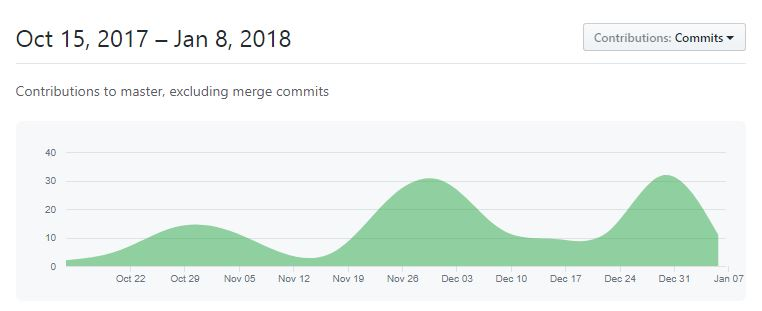
\includegraphics[width=0.8\textwidth]{Capture1.JPG}
\caption{\label{}Total number of commits over a period of time}
\end{figure}
\newline
Total lines of code - Since Json is not a language (mainly autogenerated file package-lock.json) out lines of code comes to 2276 loc.
\newline
\begin{figure}[h]
\centering
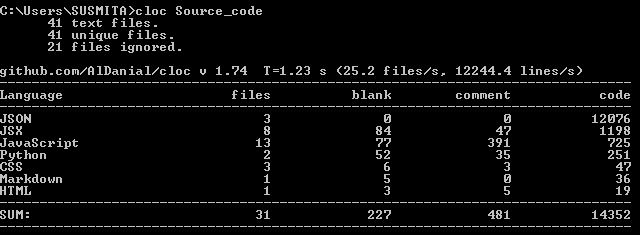
\includegraphics[width=0.8\textwidth]{Capture.JPG}
\caption{\label{}Total lines of code in the Source{\_}code.zip folder in github }
\end{figure}
\newline
We are submitting two versions of the source, a readable version and a deployable version.  A working version of the application can be found in the "web{\_}application" folder.  A non working version of the source separated into A and C can be found in Source{\_}code.zip folder.




\newpage
\section{Design and Implementation}
Initial design specifications for the prototype was to build a messaging service, following the classic chat app model such as WhatsApp or Skype. We aimed at building separate chat accounts for parents, as well as the child. After few weeks of development, we concluded that this was beyond the scope within  the given time frame. So, we came up with a model where the parent creates the account and then locks the channels and contacts. The child would then be unable to add contacts on his own.
The first step towards this was to choose an existing sdk, rather than building a messaging service from scratch, so that we could add or modify the additional functionalities based on our requirements. Twillio was our choice. After successful implementation of twillio sdk,the front end was created using React JS supported by python.  Twilio provided storage of chat history and we used 	MongoDb to store user and other details.  It is also very important to select a proper web framework when starting on a web application. We chose flask (a lightweight Python web framework) because it is simple and light weight. In our team, some members are familiar with this framework  so we have a certain foundation about the web application framework.
Flask is very simple and easy to use because the online instructions documents is very rich. It is also compatible with Google App Engine.
\newline
There are three pages in our app. They are:
\begin{itemize}
\item Signin:The signin page of the app allows users to signin using google credentials.
\item Register:The register page allows the user to set a 4 digit lock pin.  Lock/unlock is only set by parents and child users have not access to this functionality.Once a pin is set,it allows for setting a chat channel and adding friends to it.
\item Home: This is the main app page with contacts and chat window
\end{itemize}
\begin{figure}[h]
\centering
\includegraphics[width=0.8\textwidth]{FlowDiag.png}
\caption{\label{}Flow Diagram of the working system}
\end{figure}
\newpage
\section{Critical Evaluation}
\subsection{Strength}
Scalability-As described in the previous sections, we have used modern design patterns to keep our code clean, maintainable and testable.Our use of third party hosted services give our simple prototype application the ability to scale to millions of users.
\newline
Compatibility - The application uses webpack, bundled with Babel, for the javascript code. This enables our application to run on multiple browsers like Google Chrome, Firefox and Safari.
\newline
Extensibility - Additional features can be added to our app, as the code structure is easy to modify
\newline
sentiment analysis - We also made use of a hosted sentiment analysis service by IBM Watson which gave us the ability to automatically highlight messages that might be of concern.
\newline
Quick page refresh - Using React for our front end user interface allowed us to create a rich user experience that was able to refresh the display client side without the need for slow server side page refreshes.
\subsection{Challenges}
We had technical difficulties in setting up Google Datastore and instead made use of an AWS hosted instance of a mongoDB.  If we had more time we would want to replace our database with Google Datastore as it is able to provide the functionality we require and would simplify redeployment of the application.

\subsection{Market Research}
We have also done a lot of background research and market analysis to find out what exactly we want to build and why. We found that although there are a lot of similar apps in the market,none of them serves the same purpose as ours.Here is a list of apps that we found
\begin{itemize}
\item  Monster messenger:
\newline
URL-https://monster-messenger.com/
\newline
Available platform-ios,android
\newline
Target Audience-under 13
\newline
Not supported on Amazon kindle,No sentimental analysis
\item  Roo kids:
\newline
URL-http://www.rookidsapp.com/
\newline
Available platform-ios, android ,amazon kindle
\newline
No specific target audience
No sentimental analysis
\item  MMguardian:
\newline
URL-http://www.mmguardian.com/welcome-to-messenger-kids/
\newline
Available platform-android iphone
\newline
No specific target audience
\item  Facebook messenger kids:
\newline
URL-https://www.wired.com/story/facebook-for-6-year-olds-welcome-to-messenger-kids/
\newline
Available platform-ios, android ,amazon kindle
\newline
Target Audience-Target Audience-under 13
No sentimental analysis
\end{itemize}
What makes us unique is that we have an app which targets pre{-}teens(5-13) which  supports all the platforms, especially amazon kindle with sentimental analysis.
\subsection{Limitation and future work}
More testing should have been implemented with automated test suites.  Due to limitation on time and device, we did functional testing on limited browsers and devices.
\newline
For improving user experience more features could have been added like separate login and chats for parent and child. At this moment our app provides just a chat with lock button and sentimental analysis.









\end{document}